\documentclass[portrait,final,a0paper]{baposter}
%\documentclass[a4shrink,portrait,final]{baposter}
% Usa a4shrink for an a4 sized paper.

\tracingstats=2
\usepackage{calc}
\usepackage{graphicx}
\usepackage{amsmath}
\usepackage{amssymb}
\usepackage{relsize}
\usepackage{multirow}
\usepackage{bm}

\usepackage{graphicx}
\usepackage{multicol}

\usepackage{pgfbaselayers}
\pgfdeclarelayer{background}
\pgfdeclarelayer{foreground}
\pgfsetlayers{background,main,foreground}

\usepackage{times}
\usepackage{helvet}
%\usepackage{bookman}
\usepackage{palatino}
\usepackage{background}

\newcommand{\captionfont}{\footnotesize}

\selectcolormodel{cmyk}

\graphicspath{{images/}}

%%%%%%%%%%%%%%%%%%%%%%%%%%%%%%%%%%%%%%%%%%%%%%%%%%%%%%%%%%%%%%%%%%%%%%%%%%%%%%%%
%%%% Some math symbols used in the text
%%%%%%%%%%%%%%%%%%%%%%%%%%%%%%%%%%%%%%%%%%%%%%%%%%%%%%%%%%%%%%%%%%%%%%%%%%%%%%%%
% Format 
\newcommand{\Matrix}[1]{\begin{bmatrix} #1 \end{bmatrix}}
\newcommand{\Vector}[1]{\Matrix{#1}}
\newcommand*{\SET}[1]  {\ensuremath{\mathcal{#1}}}
\newcommand*{\MAT}[1]  {\ensuremath{\mathbf{#1}}}
\newcommand*{\VEC}[1]  {\ensuremath{\bm{#1}}}
\newcommand*{\CONST}[1]{\ensuremath{\mathit{#1}}}
\newcommand*{\norm}[1]{\mathopen\| #1 \mathclose\|}% use instead of $\|x\|$
\newcommand*{\abs}[1]{\mathopen| #1 \mathclose|}% use instead of $\|x\|$
\newcommand*{\absLR}[1]{\left| #1 \right|}% use instead of $\|x\|$

\def\norm#1{\mathopen\| #1 \mathclose\|}% use instead of $\|x\|$
\newcommand{\normLR}[1]{\left\| #1 \right\|}% use instead of $\|x\|$

%%%%%%%%%%%%%%%%%%%%%%%%%%%%%%%%%%%%%%%%%%%%%%%%%%%%%%%%%%%%%%%%%%%%%%%%%%%%%%%%
% Multicol Settings
%%%%%%%%%%%%%%%%%%%%%%%%%%%%%%%%%%%%%%%%%%%%%%%%%%%%%%%%%%%%%%%%%%%%%%%%%%%%%%%%
\setlength{\columnsep}{0.7em}
\setlength{\columnseprule}{0mm}


%%%%%%%%%%%%%%%%%%%%%%%%%%%%%%%%%%%%%%%%%%%%%%%%%%%%%%%%%%%%%%%%%%%%%%%%%%%%%%%%
% Save space in lists. Use this after the opening of the list
%%%%%%%%%%%%%%%%%%%%%%%%%%%%%%%%%%%%%%%%%%%%%%%%%%%%%%%%%%%%%%%%%%%%%%%%%%%%%%%%
\newcommand{\compresslist}{%
\setlength{\itemsep}{1pt}%
\setlength{\parskip}{0pt}%
\setlength{\parsep}{0pt}%
}


%\backgroundsetup{
%	scale=1,
%	color=black,
%	opacity=0.4,
%	angle=0,
%	contents={%
%  
\includegraphics[width=\paperwidth,height=\paperheight]{back}
%	}%
%}



%%%%%%%%%%%%%%%%%%%%%%%%%%%%%%%%%%%%%%%%%%%%%%%%%%%%%%%%%%%%%%%%%%%%%%%%%%%%%%
%%% Begin of Document
%%%%%%%%%%%%%%%%%%%%%%%%%%%%%%%%%%%%%%%%%%%%%%%%%%%%%%%%%%%%%%%%%%%%%%%%%%%%%%


\begin{document}
\typeout{Poster rendering started}	


%%% Setting Background Image %%%%%%%%%%%%%%%%%%%%%%%%%%%%%%%%%%%%%%%%%%%%%%%%%%
\background{
	\begin{tikzpicture}[remember picture,overlay]%
	\draw (current page.north west)+(-2em,2em) node[anchor=north west,opacity=0.3]
	{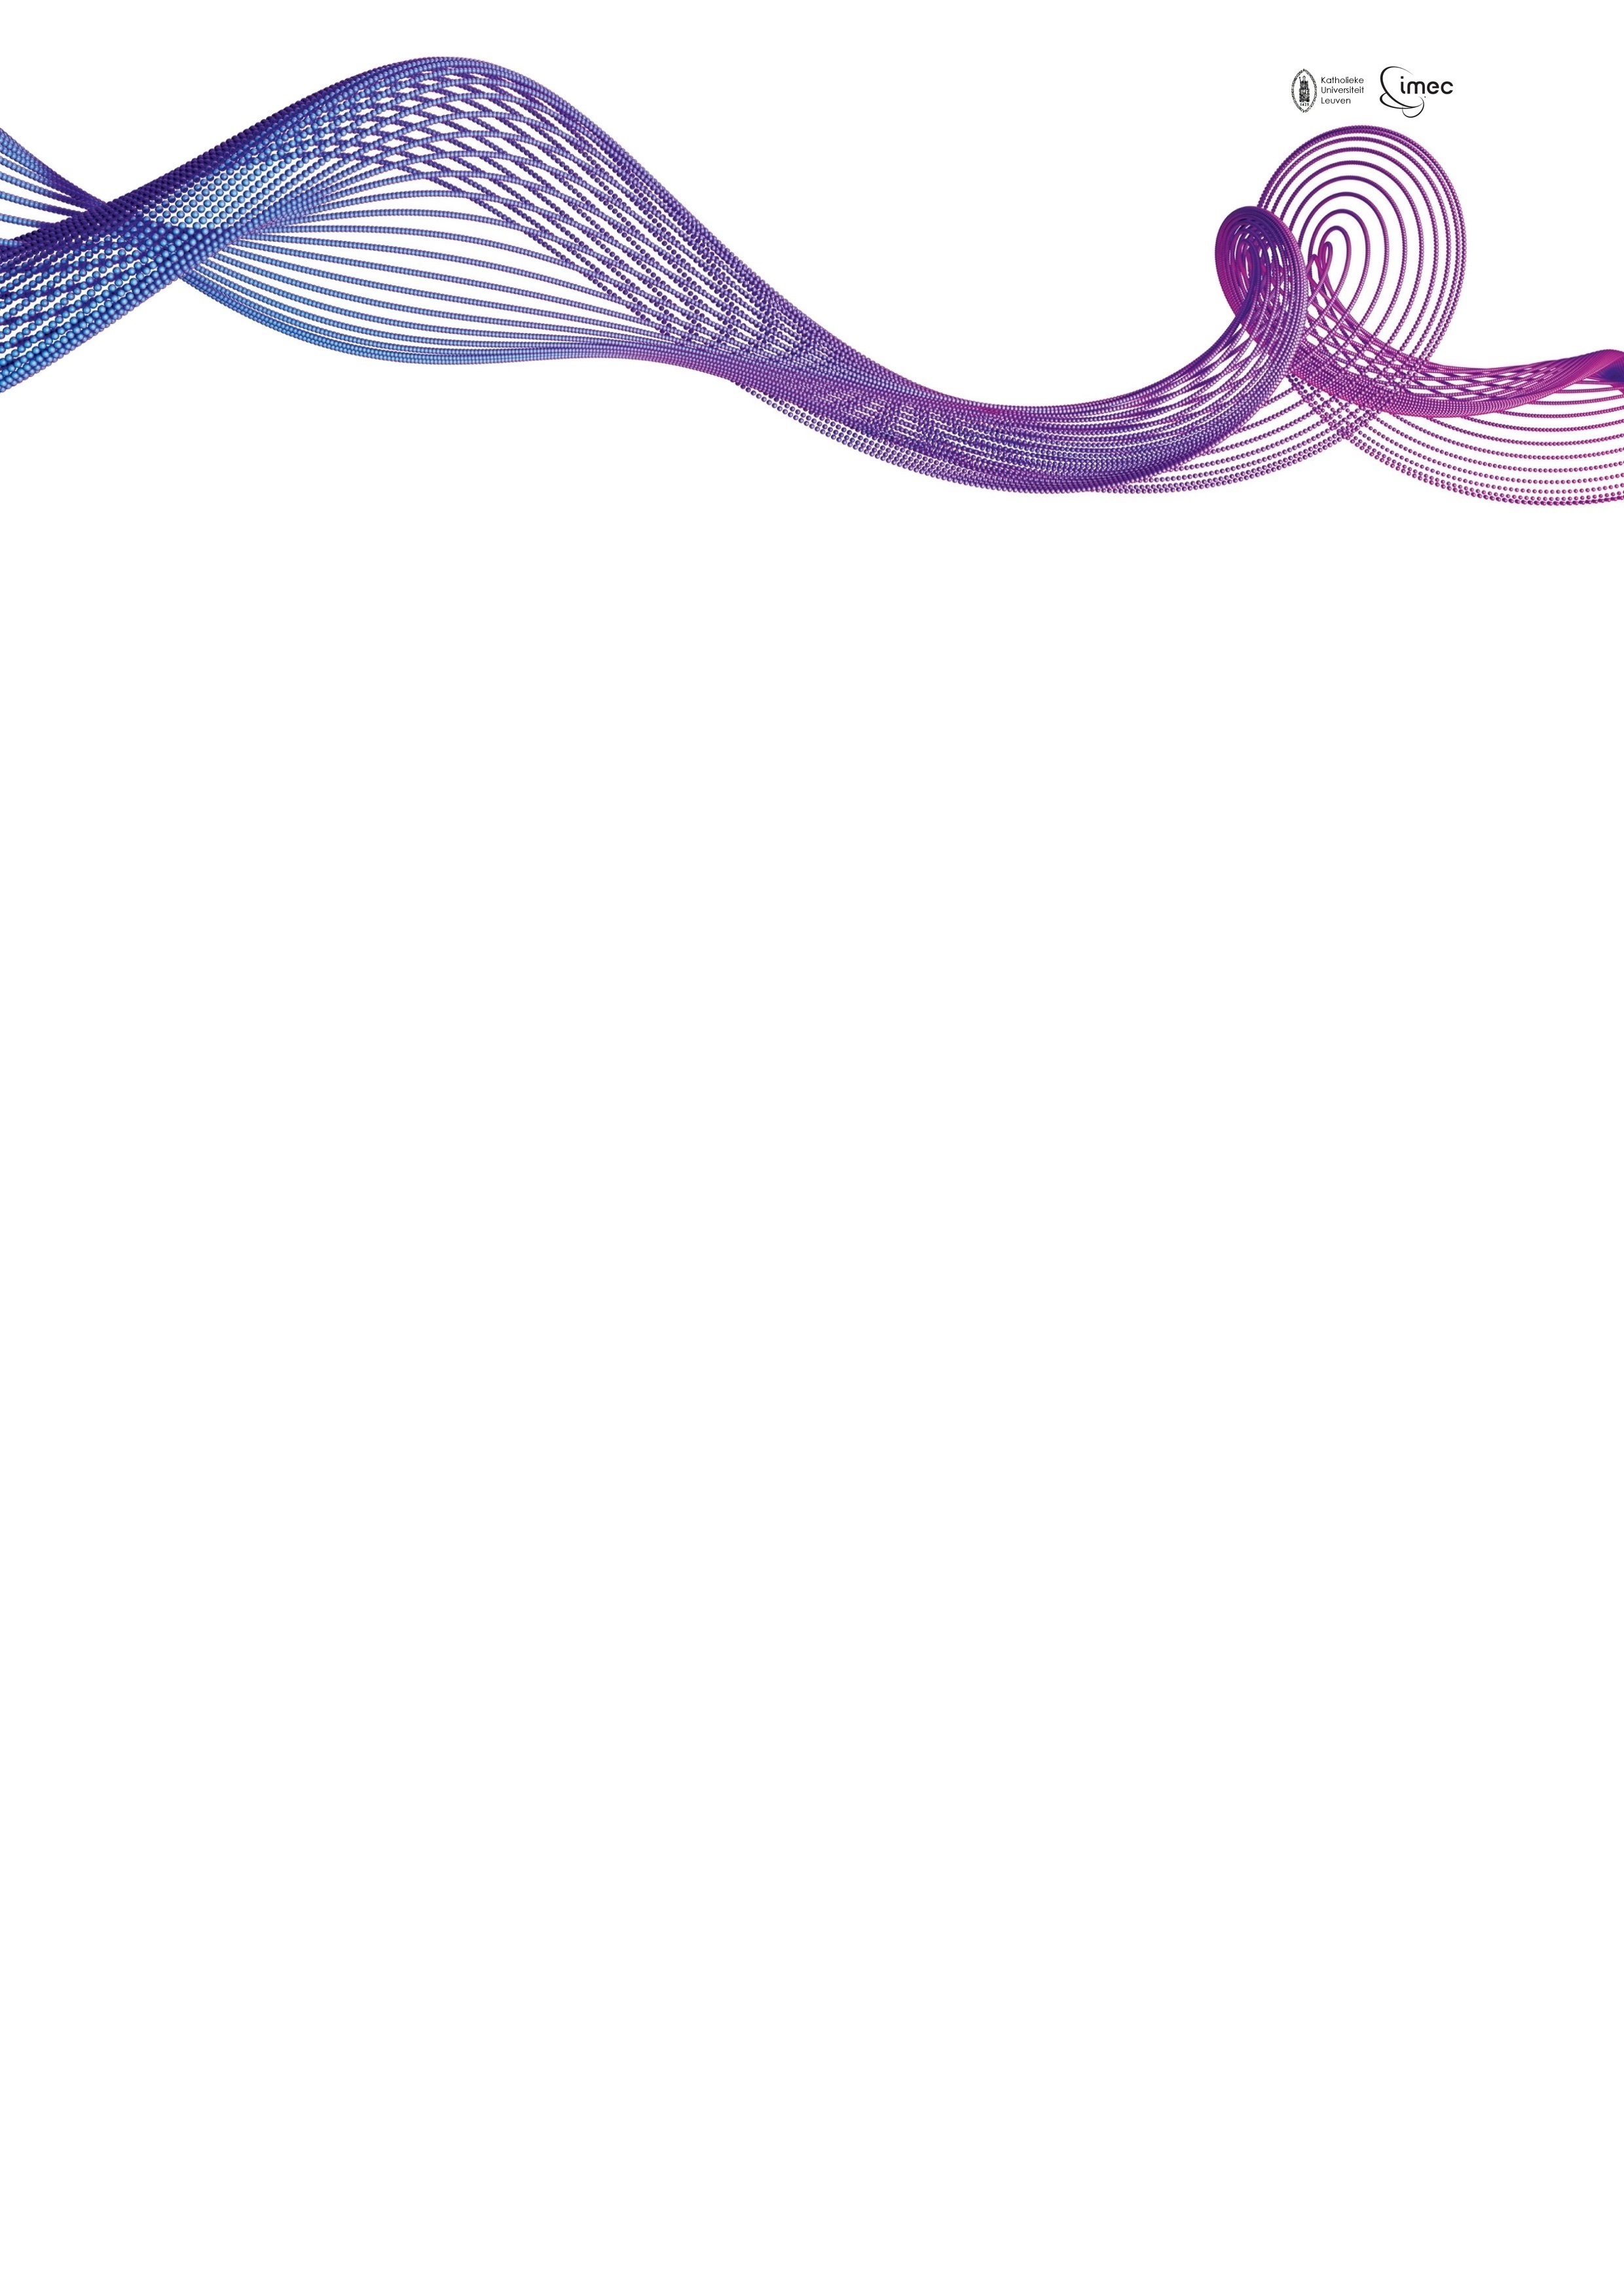
\includegraphics[height=1.1\textheight]{backCopy}};
	\end{tikzpicture}
}	

%%%%%%%%%%%%%%%%%%%%%%%%%%%%%%%%%%%%%%%%%%%%%%%%%%%%%%%%%%%%%%%%%%%%%%%%%%%%%%
%%% Here starts the poster
%%%---------------------------------------------------------------------------
%%% Format it to your taste with the options
%%%%%%%%%%%%%%%%%%%%%%%%%%%%%%%%%%%%%%%%%%%%%%%%%%%%%%%%%%%%%%%%%%%%%%%%%%%%%%
% Define some colors
\definecolor{DarkMagenta}{cmyk}{0,0.64,0.2,0}
\definecolor{yellow}{cmyk}{0.3,0.1,0.2,0.0}
\definecolor{reddishyellow}{cmyk}{0,0.22,1.0,0.0}
\definecolor{black}{cmyk}{0,0,0.0,1.0}
\definecolor{darkYellow}{cmyk}{0,0,1.0,0.5}
\definecolor{Carnelian}{cmyk}{1.0,0.29,0.0,0.26}

\definecolor{lightyellow}{cmyk}{0.0,0.0,0.0,0.0}
\definecolor{lighteryellow}{cmyk}{0,0,0.0,0.0}
\definecolor{lighteryellow}{cmyk}{0,0,0.0,0.0}
\definecolor{lightestyellow}{cmyk}{0,0,0.0,0.0}

%%
%\typeout{Poster Starts}

\newlength{\leftimgwidth}
\begin{poster}%
  % Poster Options
  {
  % Show grid to help with alignment
  grid=false,
  % Column spacing
  colspacing=1em,
  % Color style
  bgColorOne=lightestyellow,
  bgColorTwo=lightestyellow,
  borderColor=blue,
  headerColorOne=blue,
  headerColorTwo=reddishyellow,
  headerFontColor=white,
  boxColorOne=lightyellow,
  boxColorTwo=lighteryellow,
  % Format of textbox
  textborder=roundedleft,
%  textborder=rectangle,
  % Format of text header
  eyecatcher=false,
  headerborder=open,
  headerheight=0.08\textheight,
  headershape=roundedright,
  headershade=plain,
  headerfont=\Large\sf\bf, %Sans Serif
 % boxshade=plain,
%  background=shade-tb,
  background=user,
  linewidth=2pt
  }
  % Eye Catcher
  {
\includegraphics[width=10em]{back}} % No eye catcher for this poster. (eyecatcher=no above). If an eye catcher is present, the title is centered between eye-catcher and logo.
  % Title
  {\sf %Sans Serif
  %\bf% Serif
  Classification of Cells Based on Scale-space Measures and Semi-supervised machine Learning}
  % Authors
  {\sf %Sans Serif
  % Serif
  \vspace{1em}\ S. Vohra\textsuperscript{1,2}, L. Antanas\textsuperscript{2}, L. Raedt\textsuperscript{2} and D. Prodanov\textsuperscript{1}
  }
  % University logo
  {% The makebox allows the title to flow into the logo, this is a hack because of the L shaped logo.
    
  }
   

  \tikzstyle{light shaded}=[top color=baposterBGtwo!30!white,bottom color=baposterBGone!30!white,shading=axis,shading angle=30]

  % Width of left inset image
     \setlength{\leftimgwidth}{0.78em+8.0em}

%%%%%%%%%%%%%%%%%%%%%%%%%%%%%%%%%%%%%%%%%%%%%%%%%%%%%%%%%%%%%%%%%%%%%%%%%%%%%%
%%% Now define the boxes that make up the poster
%%%---------------------------------------------------------------------------
%%% Each box has a name and can be placed absolutely or relatively.
%%% The only inconvenience is that you can only specify a relative position 
%%% towards an already declared box. So if you have a box attached to the 
%%% bottom, one to the top and a third one which should be in between, you 
%%% have to specify the top and bottom boxes before you specify the middle 
%%% box.
%%%%%%%%%%%%%%%%%%%%%%%%%%%%%%%%%%%%%%%%%%%%%%%%%%%%%%%%%%%%%%%%%%%%%%%%%%%%%%
    %
    % A coloured circle useful as a bullet with an adjustably strong filling
    \newcommand{\colouredcircle}[1]{%
      \tikz{\useasboundingbox (-0.2em,-0.32em) rectangle(0.2em,0.32em); \draw[draw=black,fill=baposterBGone!80!black!#1!white,line width=0.03em] (0,0) circle(0.18em);}}

%%%%%%%%%%%%%%%%%%%%%%%%%%%%%%%%%%%%%%%%%%%%%%%%%%%%%%%%%%%%%%%%%%%%%%%%%%%%%%
  \headerbox{Introduction}{name=contribution,column=0,row=0}{
%%%%%%%%%%%%%%%%%%%%%%%%%%%%%%%%%%%%%%%%%%%%%%%%%%%%%%%%%%%%%%%%%%%%%%%%%%%%%%
 \vspace{0.3em}
   {}Morphometric analysis and identification of different phenotypes of brain cells has become increasingly important. Accurate identification of individual cellular phenotypes can be obtained by combining automated microscopic acquisition with 
   extensive morphological feature extraction and data mining strategies. Segmentation of touching cells, or cells having branching structures presents a major challenge for \textsl{intensity threshold}-based techniques. 
   Multiscale and a semi-supervised active learning-based approaches appear to be very promising in a variety of applications. We combined both the approaches to classify brain cells in a robust manner involving little human attention.
  \vspace{0.3em}
 }



%%%%%%%%%%%%%%%%%%%%%%%%%%%%%%%%%%%%%%%%%%%%%%%%%%%%%%%%%%%%%%%%%%%%%%%%%%%%%%
  \headerbox{Features}{name=resultsneutralization,column=1,row=0,span=2}{
%%%%%%%%%%%%%%%%%%%%%%%%%%%%%%%%%%%%%%%%%%%%%%%%%%%%%%%%%%%%%%%%%%%%%%%%%%%%%%
\vspace{0.3em}
Interactions of the Gaussian kernels with the image can be combined with smoothing in one step.The resulting kernel is also known as the Mexican hat filter or
1. Laplacian of Gaussian (LoG).
2. Anisotropic decomposition of LoG (ALoG).
3. Gaussian Derivative.

 \begin{minipage}{.4\textwidth}
 	\color{Carnelian}
 	\vspace{0.3em}
 	\begin{flalign*}
 	\mathrm{LoG}_s \,(r) & =-\frac{\left( 2\,s-{r}^{2}\right) \,{e}^{-\frac{{r}^{2}}{2\,s}}}{2\,\pi \,{s}^{3}}  \\
 	\end{flalign*}
 \end{minipage}
  \begin{minipage}{.72\textwidth}
  	\vspace{0.3em}
  	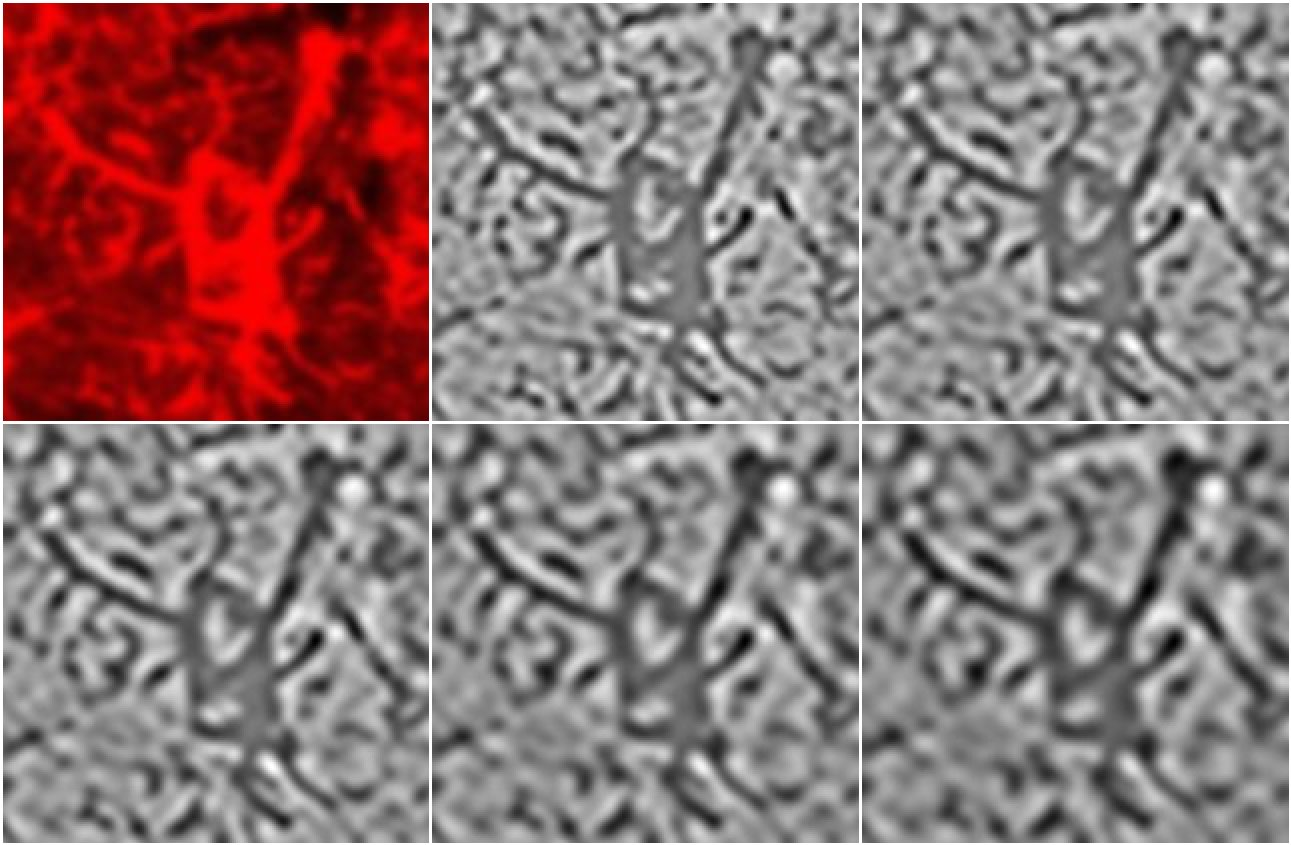
\includegraphics[width=.72\textwidth]{LOGMontage}
  	\vspace{0.4cm}
  \end{minipage}
   \color{DarkMagenta} Scale space projection of Astrocytes. Left: LoG operator zero set: Right: LoG operator equation.  
  Scales, \textit{s}=8, 10, 12, 14, 16 pixels.

  }


%%%%%%%%%%%%%%%%%%%%%%%%%%%%%%%%%%%%%%%%%%%%%%%%%%%%%%%%%%%%%%%%%%%%%%%%%%%%%%
  \headerbox{Anisotropic decomposition of LoG}{name=robustness,column=0,row=0,span=3,below=resultsneutralization}{

  	The LoG operator can be decomposed into orthogonal and tangential components.
  	
  	\vspace{0.2cm}
  	 
\begin{minipage}{.5\textwidth}
	\color{Carnelian}
	\begin{equation*}
	\label{eq:scale}
	\Delta G= \Delta_\parallel G + \Delta_\perp G
	\end{equation*}
	\begin{equation*}
	\label{eq:scale}
	\Delta_\parallel G=  \frac{1}{{r_x}^{2}+{r_y}^{2}} \left({r_x}^{2} \nabla_{xx} G + 2 {r_x} {r_y}\nabla_{xy} G + {r_y}^{2} \nabla_{yy} G \right)
	\end{equation*}
	\begin{equation*}
	\label{eq:scale}
	\Delta_\perp G=  \frac{1}{{r_x}^{2}+{r_y}^{2}} \left({r_x}^{2} \nabla_{xx} G - 2 {r_x} {r_y}\nabla_{xy} G + {r_y}^{2} \nabla_{yy} G \right)
	\end{equation*}
	\begin{equation*}
	{r_x}= \nabla_{x} G , {r_y}= \nabla_{y} G
	\end{equation*}	
\end{minipage}
\begin{minipage}{.64\textwidth}
	\includegraphics[width=.64\textwidth]{ALOGMontage} 
	 \vspace{0.4cm}
\end{minipage}
  
 \color{DarkMagenta} Scale space projection of Astrocytes. TOP: ALoG Orthogonal operator zero set: BOTTOM: ALoG tangential operator. Scales, \textit{s}=8, 10, 12, 14, 16 pixels.
  
}  

%%%%%%%%%%%%%%%%%%%%%%%%%%%%%%%%%%%%%%%%%%%%%%%%%%%%%%%%%%%%%%%%%%%%%%%%%%%%%%
\headerbox{Semi-supervised Machine Learning}{name=results,column=0,span=3,below=robustness}{
	%%%%%%%%%%%%%%%%%%%%%%%%%%%%%%%%%%%%%%%%%%%%%%%%%%%%%%%%%%%%%%%%%%%%%%%%%%%%%%
	\begin{multicols}{2}
		The method was evaluated on the GavabDB expression dataset which contains 427 Scans, with 3 neutral scans and 4 expression scans per ID.
	\end{multicols}\vspace{-1em}
	
	% \mbox{\hspace{0.3\linewidth}\rule{0.4\linewidth}{1pt}\hspace{0.3\linewidth}}\\
	% \begin{tabular}{cc}
	%  \hspace{-0.5em}\scalebox{0.735}{% GNUPLOT: LaTeX picture with Postscript
\begingroup
  \fontfamily{phv}%
  \selectfont
  \makeatletter
  \providecommand\color[2][]{%
    \GenericError{(gnuplot) \space\space\space\@spaces}{%
      Package color not loaded in conjunction with
      terminal option `colourtext'%
    }{See the gnuplot documentation for explanation.%
    }{Either use 'blacktext' in gnuplot or load the package
      color.sty in LaTeX.}%
    \renewcommand\color[2][]{}%
  }%
  \providecommand\includegraphics[2][]{%
    \GenericError{(gnuplot) \space\space\space\@spaces}{%
      Package graphicx or graphics not loaded%
    }{See the gnuplot documentation for explanation.%
    }{The gnuplot epslatex terminal needs graphicx.sty or graphics.sty.}%
    \renewcommand\includegraphics[2][]{}%
  }%
  \providecommand\rotatebox[2]{#2}%
  \@ifundefined{ifGPcolor}{%
    \newif\ifGPcolor
    \GPcolortrue
  }{}%
  \@ifundefined{ifGPblacktext}{%
    \newif\ifGPblacktext
    \GPblacktexttrue
  }{}%
  % define a \g@addto@macro without @ in the name:
  \let\gplgaddtomacro\g@addto@macro
  % define empty templates for all commands taking text:
  \gdef\gplbacktext{}%
  \gdef\gplfronttext{}%
  \makeatother
  \ifGPblacktext
    % no textcolor at all
    \def\colorrgb#1{}%
    \def\colorgray#1{}%
  \else
    % gray or color?
    \ifGPcolor
      \def\colorrgb#1{\color[rgb]{#1}}%
      \def\colorgray#1{\color[gray]{#1}}%
      \expandafter\def\csname LTw\endcsname{\color{white}}%
      \expandafter\def\csname LTb\endcsname{\color{black}}%
      \expandafter\def\csname LTa\endcsname{\color{black}}%
      \expandafter\def\csname LT0\endcsname{\color[rgb]{1,0,0}}%
      \expandafter\def\csname LT1\endcsname{\color[rgb]{0,1,0}}%
      \expandafter\def\csname LT2\endcsname{\color[rgb]{0,0,1}}%
      \expandafter\def\csname LT3\endcsname{\color[rgb]{1,0,1}}%
      \expandafter\def\csname LT4\endcsname{\color[rgb]{0,1,1}}%
      \expandafter\def\csname LT5\endcsname{\color[rgb]{1,1,0}}%
      \expandafter\def\csname LT6\endcsname{\color[rgb]{0,0,0}}%
      \expandafter\def\csname LT7\endcsname{\color[rgb]{1,0.3,0}}%
      \expandafter\def\csname LT8\endcsname{\color[rgb]{0.5,0.5,0.5}}%
    \else
      % gray
      \def\colorrgb#1{\color{black}}%
      \def\colorgray#1{\color[gray]{#1}}%
      \expandafter\def\csname LTw\endcsname{\color{white}}%
      \expandafter\def\csname LTb\endcsname{\color{black}}%
      \expandafter\def\csname LTa\endcsname{\color{black}}%
      \expandafter\def\csname LT0\endcsname{\color{black}}%
      \expandafter\def\csname LT1\endcsname{\color{black}}%
      \expandafter\def\csname LT2\endcsname{\color{black}}%
      \expandafter\def\csname LT3\endcsname{\color{black}}%
      \expandafter\def\csname LT4\endcsname{\color{black}}%
      \expandafter\def\csname LT5\endcsname{\color{black}}%
      \expandafter\def\csname LT6\endcsname{\color{black}}%
      \expandafter\def\csname LT7\endcsname{\color{black}}%
      \expandafter\def\csname LT8\endcsname{\color{black}}%
    \fi
  \fi
  \setlength{\unitlength}{0.0500bp}%
  \begin{picture}(5760.00,2520.00)%
    \gplgaddtomacro\gplbacktext{%
      \csname LTb\endcsname%
      \put(810,540){\makebox(0,0)[r]{\strut{} 75}}%
      \csname LTb\endcsname%
      \put(810,828){\makebox(0,0)[r]{\strut{} 80}}%
      \csname LTb\endcsname%
      \put(810,1116){\makebox(0,0)[r]{\strut{} 85}}%
      \csname LTb\endcsname%
      \put(810,1404){\makebox(0,0)[r]{\strut{} 90}}%
      \csname LTb\endcsname%
      \put(810,1692){\makebox(0,0)[r]{\strut{} 95}}%
      \csname LTb\endcsname%
      \put(810,1980){\makebox(0,0)[r]{\strut{} 100}}%
      \csname LTb\endcsname%
      \put(918,360){\makebox(0,0){\strut{} 0}}%
      \csname LTb\endcsname%
      \put(1372,360){\makebox(0,0){\strut{} 2}}%
      \csname LTb\endcsname%
      \put(1825,360){\makebox(0,0){\strut{} 4}}%
      \csname LTb\endcsname%
      \put(2279,360){\makebox(0,0){\strut{} 6}}%
      \csname LTb\endcsname%
      \put(2732,360){\makebox(0,0){\strut{} 8}}%
      \csname LTb\endcsname%
      \put(3186,360){\makebox(0,0){\strut{} 10}}%
      \csname LTb\endcsname%
      \put(3640,360){\makebox(0,0){\strut{} 12}}%
      \csname LTb\endcsname%
      \put(4093,360){\makebox(0,0){\strut{} 14}}%
      \csname LTb\endcsname%
      \put(4547,360){\makebox(0,0){\strut{} 16}}%
      \csname LTb\endcsname%
      \put(5000,360){\makebox(0,0){\strut{} 18}}%
      \csname LTb\endcsname%
      \put(5454,360){\makebox(0,0){\strut{} 20}}%
      \put(180,1260){\rotatebox{90}{\makebox(0,0){\strut{}MNCG \%}}}%
      \put(3186,90){\makebox(0,0){\strut{}$@(x)$}}%
      \put(3186,2250){\makebox(0,0){\strut{}\bf \normalsize GavabDB: Mean Normalized Cumulative Gain}}%
    }%
    \gplgaddtomacro\gplfronttext{%
      \csname LTb\endcsname%
      \put(4635,873){\makebox(0,0)[r]{\strut{}neutral model}}%
      \csname LTb\endcsname%
      \put(4635,693){\makebox(0,0)[r]{\strut{}expression model}}%
    }%
    \gplbacktext
    \put(0,0){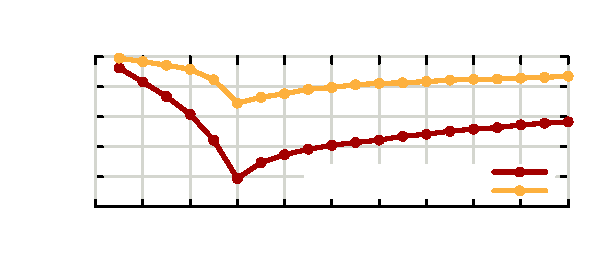
\includegraphics{shrec_mncg}}%
    \gplfronttext
  \end{picture}%
\endgroup
} &
	%  \hspace{0.5em}\scalebox{0.735}{\input{und_mncg}}
	% \end{tabular}\\
	\centering
	{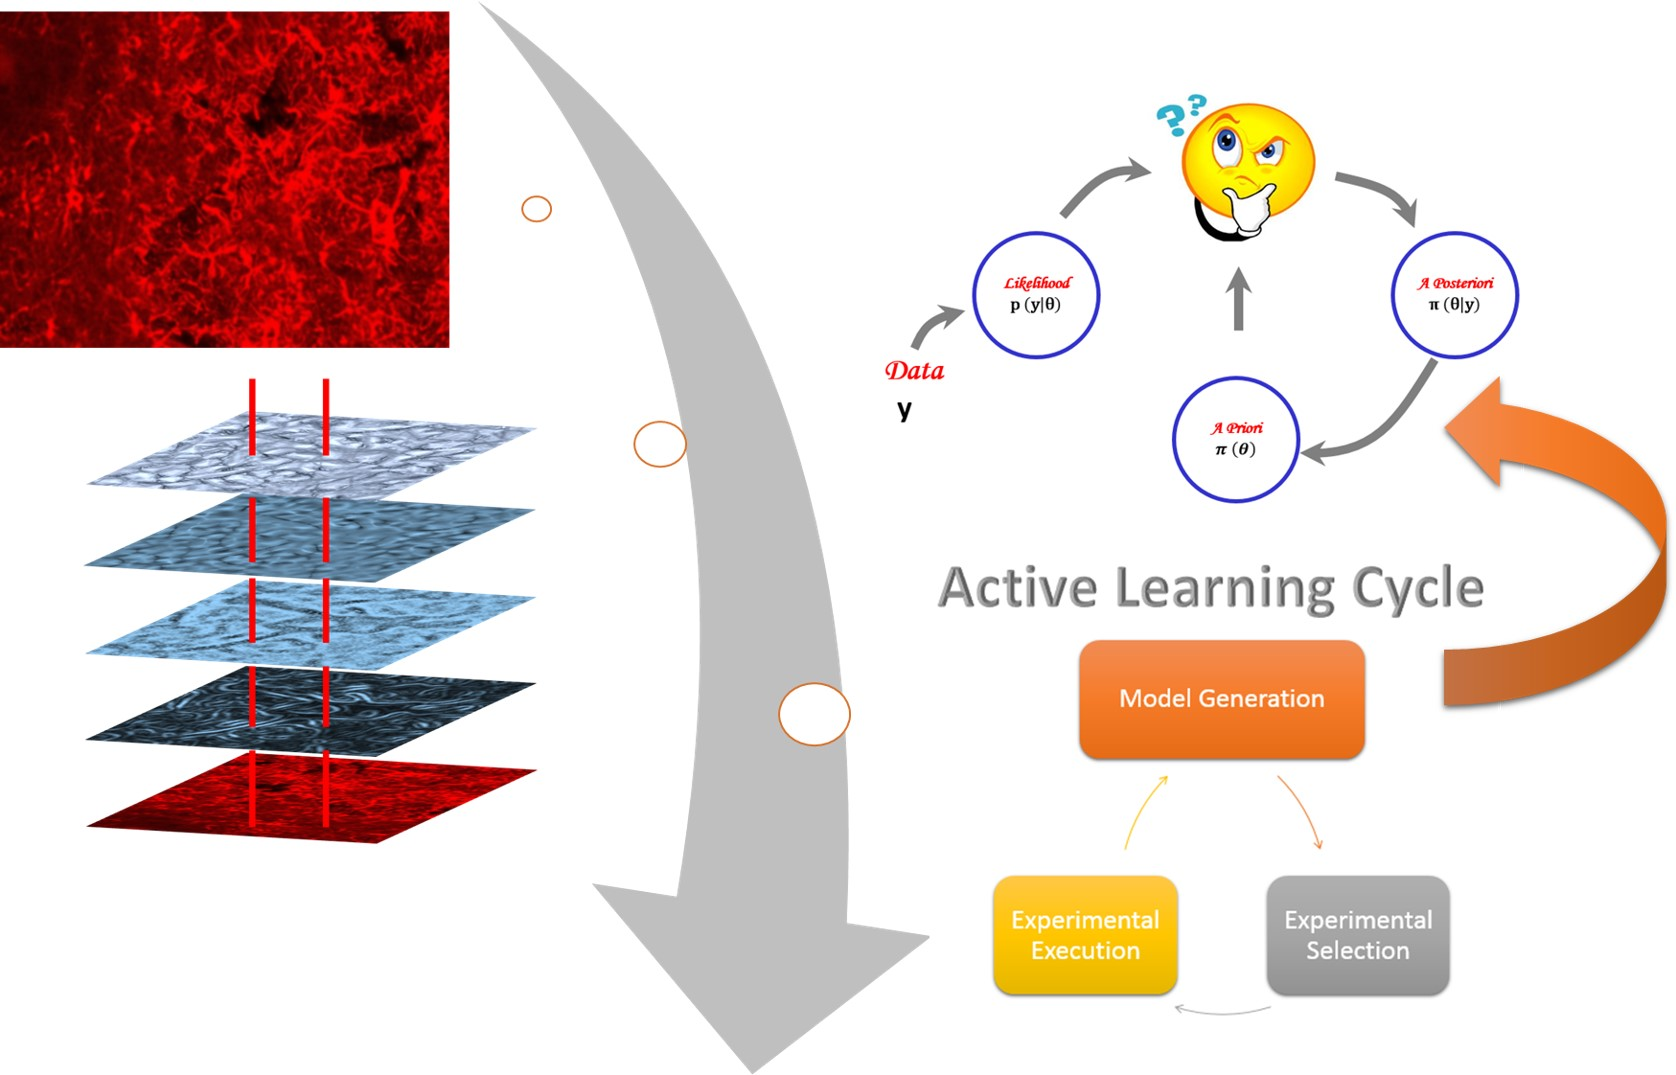
\includegraphics[height=0.31\textheight]{Results1}};    
	
	%  \vspace{0.5em}
}

%%%%%%%%%%%%%%%%%%%%%%%%%%%%%%%%%%%%%%%%%%%%%%%%%%%%%%%%%%%%%%%%%%%%%%%%%%%%%%
\headerbox{Conclusion}{name=funding,column=0,span=3,below=results}{
	%%%%%%%%%%%%%%%%%%%%%%%%%%%%%%%%%%%%%%%%%%%%%%%%%%%%%%%%%%%%%%%%%%%%%%%%%%%%%%
	\smaller 
	\hspace{1em}This work was supported in part by Microsoft Research through the European PhD Scholarship Programme.
}

\end{poster}

\end{document}
